\documentclass[11pt]{article}
\usepackage[T1]{fontenc}
\usepackage[a4paper,margin=1in]{geometry}
\usepackage{amsmath,amssymb,amsthm}
\usepackage{graphicx}
\usepackage[hidelinks]{hyperref}
\usepackage{microtype}

\newtheorem{theorem}{Theorem}
\newtheorem{lemma}{Lemma}
\newtheorem*{sourcequestion}{Proposed relation in Section 1.1}
\newtheorem*{remark}{Scope remark}

\newcommand{\N}{\mathbb N}
\newcommand{\R}{\mathbb R}
\newcommand{\Lop}{\mathcal L}
\newcommand{\Bop}{\mathbb L}
\newcommand{\G}{\mathcal G}
\newcommand{\Hspace}{\mathcal H}

\setlength{\parindent}{0pt}
\setlength{\parskip}{0.5em}

\title{A Unique Maximal Eigenmeasure but an\\
Infinite-Dimensional Bidual Ruelle Eigenspace}
\author{Run \texttt{fa\_banach\_001}, lane 17 (\texttt{agent\_lane\_17})}
\date{13 August 2026}

\begin{document}
\maketitle

\begin{center}
\fbox{\parbox{0.9\textwidth}{
\textbf{Status: full negative answer, likely valid, pending human review.}
For the fair two-symbol Bernoulli shift with zero potential, the maximal
eigenmeasure is unique, but the eigenspace of the double transpose on
$L^1(\nu)^{**}$ is infinite-dimensional.
}}
\end{center}

\section{Exact source question}

Cioletti, van Enter, and Ruviaro study the natural extension
$\Bop_f:L^1(\nu)\to L^1(\nu)$ of a Ruelle operator.  In Section 1.1,
arXiv PDF page 4 of~\cite{source}, they consider the barycenter $\nu$ of
$\G^*(f)$ and ask about the relation

\begin{sourcequestion}
\[
 \dim_{\R}\Hspace=\#\operatorname{ex}(\G^*(f)),
 \qquad
 \Hspace=\{\xi\in L^1(\nu)^{**}:
        \Bop_f^{**}\xi=\rho(\Lop_f)\xi\}.
\]
\end{sourcequestion}

The exact passage is reproduced below.

\begin{center}
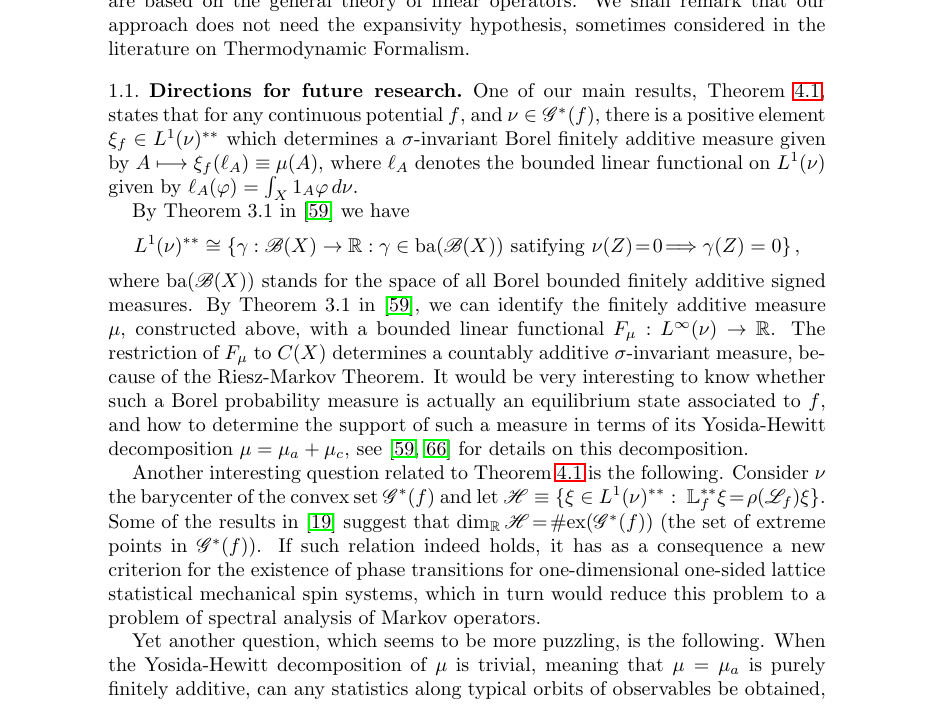
\includegraphics[width=0.92\textwidth]{figures/dimension_question_crop.png}
\end{center}

We give a counterexample in the simplest possible symbolic system.  In fact,
the left-hand side is infinite while the right-hand side equals one.

\section{The zero-potential Bernoulli system}

Let $E=\{0,1\}$, let $p=\tfrac12(\delta_0+\delta_1)$, put
$X=E^{\N}$, and write $\sigma:X\to X$ for the left shift.  Take $f=0$.
Then
\[
 (\Lop\varphi)(x)=\frac12\varphi(0x)+\frac12\varphi(1x),
 \qquad \varphi\in C(X),
 \tag{1}\label{eq:ruelle}
\]
and $\rho(\Lop)=1$.

\begin{lemma}\label{lem:unique}
The set of maximal eigenmeasures is the singleton
\[
 \G^*(0)=\{\nu\},\qquad
 \nu=\left(\tfrac12\delta_0+\tfrac12\delta_1\right)^{\N}.
\]
Consequently $\#\operatorname{ex}(\G^*(0))=1$, and its barycenter is $\nu$.
\end{lemma}

\begin{proof}
Since $\Lop 1=1$ and $\|\Lop\|=1$, the spectral radius is one.  If a Borel
probability measure $m$ satisfies $\Lop^*m=m$, then for every binary word
$w=w_1\ldots w_n$, whose cylinder is denoted $[w]$, equation
\eqref{eq:ruelle} gives
\[
 \Lop 1_{[w]}=\frac12 1_{[w_2\ldots w_n]}.
\]
(For $n=1$, the last indicator is $1$.)  Hence
$m([w])=2^{-1}m([w_2\ldots w_n])=2^{-n}$.  Cylinder probabilities determine
the measure, so $m=\nu$.  Conversely, the product measure plainly is fixed.
\end{proof}

Let $\Bop:L^1(\nu)\to L^1(\nu)$ be the natural extension of \eqref{eq:ruelle}.
It is a positive contraction.  Under the identification
$L^1(\nu)^*=L^\infty(\nu)$, its adjoint is the Koopman isometry
\[
 U\psi=\psi\circ\sigma.
 \tag{2}\label{eq:adjoint}
\]
Indeed, first for bounded measurable functions and then by density,
\[
 \int_X(\Bop h)\psi\,d\nu
 =\int_X h(\psi\circ\sigma)\,d\nu.
\]
Thus $\Bop^{**}=U^*$ on $L^1(\nu)^{**}=L^\infty(\nu)^*$.

\section{Periodic-orbit states in the bidual}

Fix a periodic point $y\in X$.  Let $C_n(y)$ be the cylinder consisting of
sequences whose first $n$ coordinates agree with those of $y$.  Since
$\nu(C_n(y))=2^{-n}$, define a positive norm-one functional on
$L^\infty(\nu)$ by
\[
 \lambda_n^y(\psi)=2^n\int_{C_n(y)}\psi\,d\nu.
 \tag{3}\label{eq:concentration}
\]
Banach--Alaoglu gives a weak-star cluster point $\lambda_y$ of this net in
$L^\infty(\nu)^*$.  If $\varphi\in C(X)$, uniform continuity and the fact
that the diameters of $C_n(y)$ tend to zero imply
\[
 \lambda_y(\varphi)=\varphi(y).
 \tag{4}\label{eq:evaluation}
\]
Thus $\lambda_y$ is an $L^\infty(\nu)^*$-state extending evaluation at the
$\nu$-null point $y$ on the continuous subspace.

Now form the Ces\`aro averages
\[
 A_N^y=\frac1N\sum_{j=0}^{N-1}(U^*)^j\lambda_y.
 \tag{5}\label{eq:cesaro}
\]
They are again positive norm-one functionals.  Take a weak-star cluster point
$\eta_y$.  Since
\[
 \|U^*A_N^y-A_N^y\|
 \le \frac{\|(U^*)^N\lambda_y\|+\|\lambda_y\|}{N}
 \le \frac2N,
\]
we have $U^*\eta_y=\eta_y$, so $\eta_y\in\Hspace$.

If the orbit $O(y)$ has period $r$, equations \eqref{eq:adjoint},
\eqref{eq:evaluation}, and \eqref{eq:cesaro} show that on $C(X)$,
\[
 \eta_y(\varphi)
 =\lim_{N\to\infty}\frac1N\sum_{j=0}^{N-1}\varphi(\sigma^j y)
 =\frac1r\sum_{z\in O(y)}\varphi(z).
 \tag{6}\label{eq:orbitmeasure}
\]
Thus the restriction of $\eta_y$ is precisely the uniform probability
measure on the periodic orbit.

\begin{theorem}\label{thm:counterexample}
For the system above, $\Hspace$ is infinite-dimensional even though
$\#\operatorname{ex}(\G^*(0))=1$.  Hence the proposed dimension relation is
false.
\end{theorem}

\begin{proof}
For $m\ge1$, let $y^{(m)}=(10^m)^{\infty}$.  These points belong to pairwise
distinct periodic orbits $O_m$.  Construct $\eta_m:=\eta_{y^{(m)}}$ as
above.  Suppose that a finite linear combination
$\sum_{m\in F}a_m\eta_m$ vanishes.  For any fixed $k\in F$, the finite
closed sets $O_k$ and $\bigcup_{m\in F\setminus\{k\}}O_m$ are disjoint, so
there is a continuous function $\varphi_k$ equal to one on $O_k$ and zero on
all the other orbits.  Restricting the relation to $C(X)$ and using
\eqref{eq:orbitmeasure} gives $a_k=0$.  Hence the family $(\eta_m)_{m\ge1}$
is linearly independent in $\Hspace$.

Lemma~\ref{lem:unique} gives the claimed value one on the right-hand side.
\end{proof}

\section{Verification, scope, and novelty}

The construction uses only positive norm-one functionals.  The first weak-star
limit extends point evaluation from $C(X)$ to $L^\infty(\nu)$; the second
turns it into an invariant state.  Norm convergence of the coboundary in
\eqref{eq:cesaro} makes invariance independent of the chosen subnet.  Linear
independence is certified after restriction to $C(X)$, where the states are
ordinary mutually singular periodic-orbit measures.

This does not contradict uniqueness in Lemma~\ref{lem:unique}: the additional
states are finitely additive elements of $L^1(\nu)^{**}$ and do not come from
$L^1(\nu)$.  Thus a modified question restricted to the canonical
$L^1(\nu)$ copy could behave differently.

The bounded novelty search checked the run's solution, attempt, proof-gap,
and ledger indexes; the parsed local arXiv corpus; exact-title and
exact-question searches; and focused arXiv/web searches for the bidual
eigenspace dimension and finitely additive Ruelle eigenvectors.  It found the
source's 2023 publication and neighboring work on eigendistributions, but no
later explicit resolution of this dimension relation.  The invariant-mean
mechanism itself is classical in spirit, so novelty is plausible rather than
certified.  Human review should prioritize the identification
$\Bop^*=U$ and the two weak-star cluster-point passages.

\begin{thebibliography}{9}
\bibitem{source}
L. Cioletti, A. van Enter, and R. Ruviaro,
\emph{The Double Transpose of the Ruelle Operator},
Monatsh. Math. \textbf{200} (2023), 523--544;
arXiv:1710.03841v4.
\end{thebibliography}

\end{document}
